
\documentclass{article}
\usepackage{pgfplots}
\usepackage{pgfplotstable}
\usepackage{tikz}
\pgfplotsset{compat=1.8}
\begin{document}
    \begin{figure*}[t]
        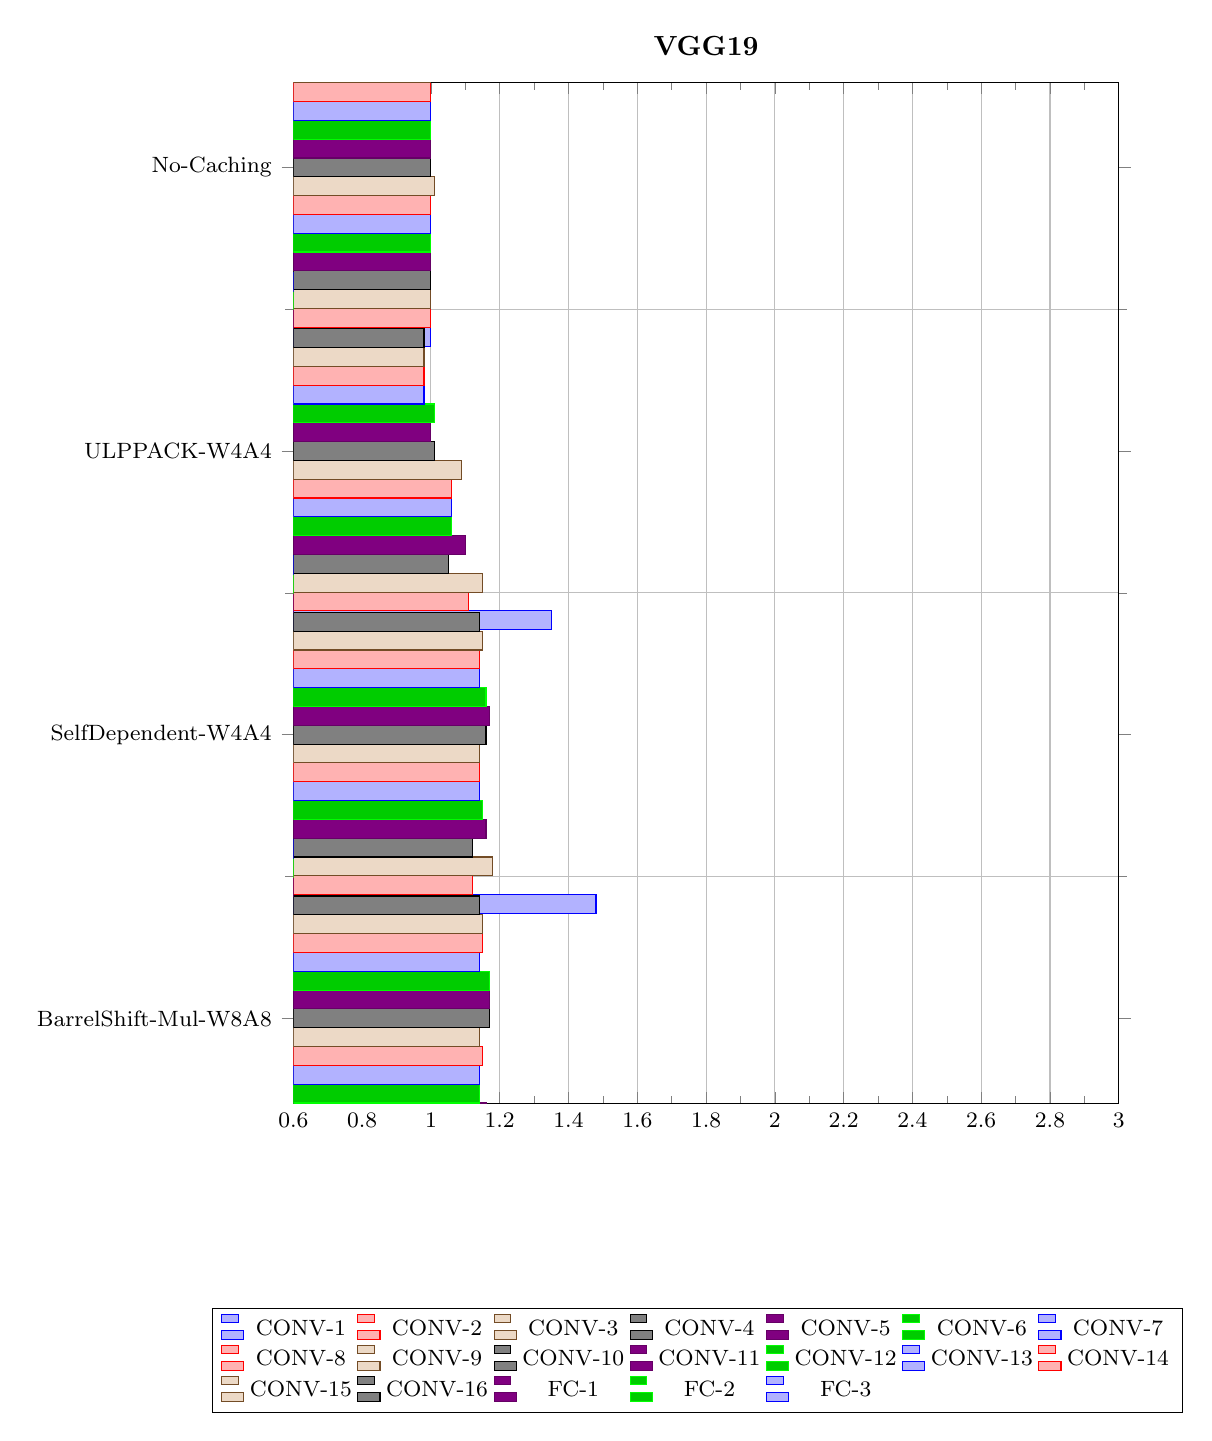
\begin{tikzpicture}
            \begin{axis}[
                xbar=0pt,
                xmin=0.6,
                xmax=3,
                width=0.995\linewidth,
                height=2*\axisdefaultheight,
                tick label style={font=\footnotesize},
                legend style={font=\tiny},
                label style={font=\footnotesize},
                symbolic y coords={BarrelShift-Mul-W8A8, SelfDependent-W4A4, ULPPACK-W4A4, No-Caching, GEMMLOWP},
                ytick=data,
                xtick={0.60,0.80,1.0,1.2,1.4,1.6,1.8,2.0,2.2,2.4,2.6,2.8,3.0},
                align={center},
                bar width=1.579ex,
                legend columns=7,
                legend style={at={(0.49,-0.2)},anchor=north,font=\footnotesize},
                title=\textbf{VGG19},
                xmajorgrids,
                yminorgrids = true,
                minor tick num=1
                ]
                \addplot coordinates { (1.49,BarrelShift-Mul-W8A8) (1.48,SelfDependent-W4A4) (1.35,ULPPACK-W4A4) (1.00,No-Caching) (0.06,GEMMLOWP) };
                \addplot coordinates { (1.13,BarrelShift-Mul-W8A8) (1.12,SelfDependent-W4A4) (1.11,ULPPACK-W4A4) (1.00,No-Caching) (0.23,GEMMLOWP) };
                \addplot coordinates { (1.18,BarrelShift-Mul-W8A8) (1.18,SelfDependent-W4A4) (1.15,ULPPACK-W4A4) (1.00,No-Caching) (0.24,GEMMLOWP) };
                \addplot coordinates { (1.12,BarrelShift-Mul-W8A8) (1.12,SelfDependent-W4A4) (1.05,ULPPACK-W4A4) (1.00,No-Caching) (0.33,GEMMLOWP) };
                \addplot coordinates { (1.16,BarrelShift-Mul-W8A8) (1.16,SelfDependent-W4A4) (1.10,ULPPACK-W4A4) (1.00,No-Caching) (0.29,GEMMLOWP) };
                \addplot coordinates { (1.14,BarrelShift-Mul-W8A8) (1.15,SelfDependent-W4A4) (1.06,ULPPACK-W4A4) (1.00,No-Caching) (0.29,GEMMLOWP) };
                \addplot coordinates { (1.14,BarrelShift-Mul-W8A8) (1.14,SelfDependent-W4A4) (1.06,ULPPACK-W4A4) (1.00,No-Caching) (0.29,GEMMLOWP) };
                \addplot coordinates { (1.15,BarrelShift-Mul-W8A8) (1.14,SelfDependent-W4A4) (1.06,ULPPACK-W4A4) (1.00,No-Caching) (0.29,GEMMLOWP) };
                \addplot coordinates { (1.14,BarrelShift-Mul-W8A8) (1.14,SelfDependent-W4A4) (1.09,ULPPACK-W4A4) (1.01,No-Caching) (0.27,GEMMLOWP) };
                \addplot coordinates { (1.17,BarrelShift-Mul-W8A8) (1.16,SelfDependent-W4A4) (1.01,ULPPACK-W4A4) (1.00,No-Caching) (0.18,GEMMLOWP) };
                \addplot coordinates { (1.17,BarrelShift-Mul-W8A8) (1.17,SelfDependent-W4A4) (1.00,ULPPACK-W4A4) (1.00,No-Caching) (0.18,GEMMLOWP) };
                \addplot coordinates { (1.17,BarrelShift-Mul-W8A8) (1.16,SelfDependent-W4A4) (1.01,ULPPACK-W4A4) (1.00,No-Caching) (0.18,GEMMLOWP) };
                \addplot coordinates { (1.14,BarrelShift-Mul-W8A8) (1.14,SelfDependent-W4A4) (0.98,ULPPACK-W4A4) (1.00,No-Caching) (0.21,GEMMLOWP) };
                \addplot coordinates { (1.15,BarrelShift-Mul-W8A8) (1.14,SelfDependent-W4A4) (0.98,ULPPACK-W4A4) (1.00,No-Caching) (0.21,GEMMLOWP) };
                \addplot coordinates { (1.15,BarrelShift-Mul-W8A8) (1.15,SelfDependent-W4A4) (0.98,ULPPACK-W4A4) (1.00,No-Caching) (0.21,GEMMLOWP) };
                \addplot coordinates { (1.14,BarrelShift-Mul-W8A8) (1.14,SelfDependent-W4A4) (0.98,ULPPACK-W4A4) (1.00,No-Caching) (0.21,GEMMLOWP) };
                \addplot coordinates { (0.32,BarrelShift-Mul-W8A8) (0.32,SelfDependent-W4A4) (0.24,ULPPACK-W4A4) (1.01,No-Caching) (0.01,GEMMLOWP) };
                \addplot coordinates { (0.32,BarrelShift-Mul-W8A8) (0.32,SelfDependent-W4A4) (0.27,ULPPACK-W4A4) (0.99,No-Caching) (0.01,GEMMLOWP) };
                \addplot coordinates { (0.33,BarrelShift-Mul-W8A8) (0.33,SelfDependent-W4A4) (0.28,ULPPACK-W4A4) (1.00,No-Caching) (0.01,GEMMLOWP) };
                \legend{
                    CONV-1,
                    CONV-2,
                    CONV-3,
                    CONV-4,
                    CONV-5,
                    CONV-6,
                    CONV-7,
                    CONV-8,
                    CONV-9,
                    CONV-10,
                    CONV-11,
                    CONV-12,
                    CONV-13,
                    CONV-14,
                    CONV-15,
                    CONV-16,
                    FC-1,
                    FC-2,
                    FC-3,
                };
            \end{axis}
        \end{tikzpicture}
    \end{figure*}
\end{document}
